\section{Opis wykorzystanych technologii}
Realizacja celu pracy wymagała wykorzystania wielu różnych technologii. Aplikacja na telefon odczytująca kody QR, musiała zostać stworzona na jeden z systemów mobilnych. Podobnie serwer wymagał wybrania konkretnego frameworku. W tym rozdziale zostały przedstawione oraz omówione użyte podejścia.

\subsection{Kody graficzne QR}
Przedstawianie danych w postaci kodów graficznych nie jest niczym innowacyjnym - w sklepach towary oznaczane są za pomocą jednowymiarowego kodu kreskowego. Kombinacja jasnych oraz ciemnych linii umożliwia przechowywanie danych, które odczytywane są za pomocą skanera z laserem. Tego typu metody stosuje się głównie w celach identyfikacji. Do przechowywania większej ilości danych wykorzystuje się częściej tzw. kody 2D.

Kody QR (ang. Quick Respone - szybka odpowiedź) to dwuwymiarowe, matrycowe, kwadratowe kody graficzne. Składają się z modułów, czyli kombinacji ciemnych oraz jasnych kwadratów, które są nośnikami danych. Zostały stworzone przez japońską firmę Denso-Wave w 1994 r \cite{thonky_tutorial}. Według postanowień licencyjnych mogą być wykorzystywane bez żadnych opłat, a sam standard jest opisany w normie ISO/IEC 18004:2015 \cite{norma_qr}. Dzięki dodatkowemu wymiarowi, pozwalają na przechowywanie większej ilości informacji (do ok. 7000 liczb lub 4000 znaków alfanumerycznych) niż kody kreskowe, posiadające tylko jeden wymiar. Ponadto, zapewniają zdecydowanie lepszą korekcję błędów. Nawet częściowo uszkodzony kod może zostać poprawnie odczytany. Posiadają kilka miejsc szczególnych do ułatwienia orientacji podczas odkodowywania. Ich liczba zależy od rozmiaru kodu.

\begin{figure}[h]
	\begin{center}
		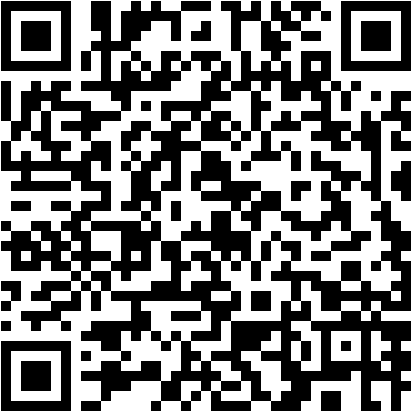
\includegraphics[width=0.2\textwidth]{02/qr_title}
	\end{center}
	\caption{Tytuł pracy przedstawiony w postaci kodu QR}
	\vspace{-0.3cm}
\end{figure}

Pierwotnie bardzo duże zastosowanie kody QR znalazły w logistyce, gdzie zawierały informacje o przesyłanych paczkach. Współcześnie kojarzone są przeważnie z urządzeniami mobilnymi. Spotykane na przystankach, w sklepach lub magazynach służą do komunikacji z użytkownikami smartfonów, przełamując niejako barierę między światem wirtualnym, a rzeczywistym. Kod zawiera informacje jedynie w postaci liczb, liter i symboli. Jednak odpowiednie formatowanie informacji, pozwala na dodatkowe interpretowanie ich przez urządzenie przenośne. I tak po zeskanowaniu może zostać wysłana wiadomość e-mail, albo dodany numer do kontaktów. Najczęściej jednak zawierają adresy URL, które powodują wyświetlenie odpowiedniej strony w przeglądarce internetowej telefonu.

% jeszcze można zrobić część o budowie kodu, gdzie wstawi się grafikę z wiki i opowie o tym z jakich elementów się składa
\subsubsection*{Sposoby kodowania, generowania oraz odczytywania}
Aby przedstawić informacje w postaci kodu QR, trzeba najpierw określić rodzaj oraz ilość danych, jakie mają zostać zakodowane. Istnieją trzy główne parametry: wersja, typ danych oraz poziom korekcji błędów.

Wersje to inaczej rozmiary kodu numerowane od 1 do 40. Decydują o ilości modułów, czyli wielkości danych jakie można przechować. Wersja pierwsza posiada 21x21 modułów, a każda kolejna jest większa o trzy na każdy bok. Maksymalny rozmiar to 177x177 dla wersji 40. 

Rodzaj kodowanych danych zależny jest od typu informacji, jaka ma być przechowywana. Ten parametr decyduje o ilości bitów przypadających na jeden znak (co wpływa na maksymalną pojemność), oraz na sposób w jaki dane mają zostać odkodowane. Możliwe są cztery sposoby kodowania:
\begin{itemize}
	\item Numeryczny -- ten tryb pozwala na zakodowanie tylko cyfr od 0 do 9, co umożliwia maksymalnie na przechowywanie 7089 znaków.
	\item Alfanumeryczny -- oprócz cyfr, także wielkie litery oraz znaki '\$', '\%', '*', '+', '-', '.', '/', ':' i spacja. Można zakodować do 4296 znaków. 
	\item Binarny -- domyślnie dla zestawu znaków z ISO-8859-1, ale także UTF-8. Maksymalnie 2953 znaków.
	\item Kanji -- znaki z systemu kodowania Shift JIS. Pomieści nie więcej niż 1817 znaków.
\end{itemize}

Poziom korekcji błędów służy do określenia, czy dane zostały odczytane poprawnie. Pozwala także na odzyskanie części z nich, nawet jeśli kod został uszkodzony (dzięki algorytmowi Reeda-Solomona). Specyfikacja wyróżnia cztery poziomy korekcji. Obok każdego z nich podany został procent danych, jakie można odzyskać:
\begin{itemize}
	\item L (Low) - 7\% danych,
	\item M (Medium) - 15\% danych,
	\item Q (Quartile) - 25\% danych,
	\item H (High) - 30\% danych.
\end{itemize}

\begin{table}[h]
	\caption{Pojemność kodów QR dla różnych ustawień}
	\vspace{0.3cm}
	\begin{center}
		\begin{tabular}{| c | c | c | c | c | c | c |}
			\hline
			Wersja & Moduły & Korekcja & Numeryczny & Alfanumeryczny & Binarny & Kanji\\
			\hline
			\multirow{4}{*}{1} & \multirow{4}{*}{21x21}&L&41&25&17&10\\
			& & M&34&20&14&8\\
			& & Q&27&16&11&7\\
			& & H&17&10&7&4\\
			\hline
			\multirow{4}{*}{40} & \multirow{4}{*}{177x177}&L&7089&4296&2953&1817\\
			& & M&5596&3391&2331&1435\\
			& & Q&3993&2420&1663&1024\\
			& & H&3057&1852&1273&784\\
			\hline
		\end{tabular}
	\end{center}
\end{table}
Istnieje wiele sposobów na generowanie kodów QR. Jednym z nich są strony www, gdzie po podaniu danych i parametrów można pobrać kod w postaci obrazka, np.: http://www.qr-code-generator.com/. Innym rozwiązaniem jest skorzystanie z gotowych bibliotek i wygenerowanie takiego kodu z poziomu języka programowania. I na przykład w Pythonie można skorzystać z modułu \textit{qrcode}.

Odczytanie, czyli odkodowanie informacji także możliwe jest na wiele sposobów. Razem z systemami mobilnymi często dostarczane są specjalne aplikacje, które wykorzystując wbudowaną kamerę, pozwalają na odczytanie zakodowanych danych. Podobnie, takie rozwiązanie możliwe jest dzięki odpowiednim biblioteką. W Androidzie jest to dostępna za darmo \textit{Zebra Crossing}.


\subsection{System Android}
% o systemach mobilnych. Procentowy udział - wykresik
% Android, krótko co to jest
% Android, krótka historia
% opisać jak to działa pod spodem. Java, kompilacja, Dalvik
Systemy na urządzenia mobilne z czasem stawały się coraz bardziej zaawansowane, przypominając swoją funkcjonalnością te przeznaczone na komputery. Dzisiaj oprócz obsługi podstawowych zadań telefonu, jak dzwonienie, pozwalają na przeglądanie internetu, czy instalowanie dodatkowych aplikacji. Do najpopularniejszych systemów w Polsce należą: Android z 65\% udziałem w rynku, Windows Phone - 16\% i iOS - 4\% \cite{polska_jest_mobi}.


\subsubsection*{O Androidzie}

Android to mobilna platforma systemowa, stworzona w 2003~r, a następnie wykupiona przez Google'a w 2005~r. z rąk niewielkiej firmy Android Inc. Od 2007~r. rozwijany jest w ramach sojuszu kilkudziesięciu firm - Open Handset Alliance. Android został zbudowany na bazie jądra Linuksa, i podobnie jak on rozpowszechniany jest za darmo z dostępnym publicznie kodem. To właśnie dostępność oraz możliwość dowolnego modyfikowania spowodowała, że zdołał w tak niedługim czasie zawładnąć rynkiem, stając się najpopularniejszym systemem mobilnym. Można go spotkać na większości popularnych urządzeń przenośnych, jak: telefony komórkowe, smartfony, tablety, netbooki. Jest stosowany także w e-bookach niektórych firm, czy innych sprzętach domowego użytku. 

%\begin{figure}[h]
%	\begin{center}
%		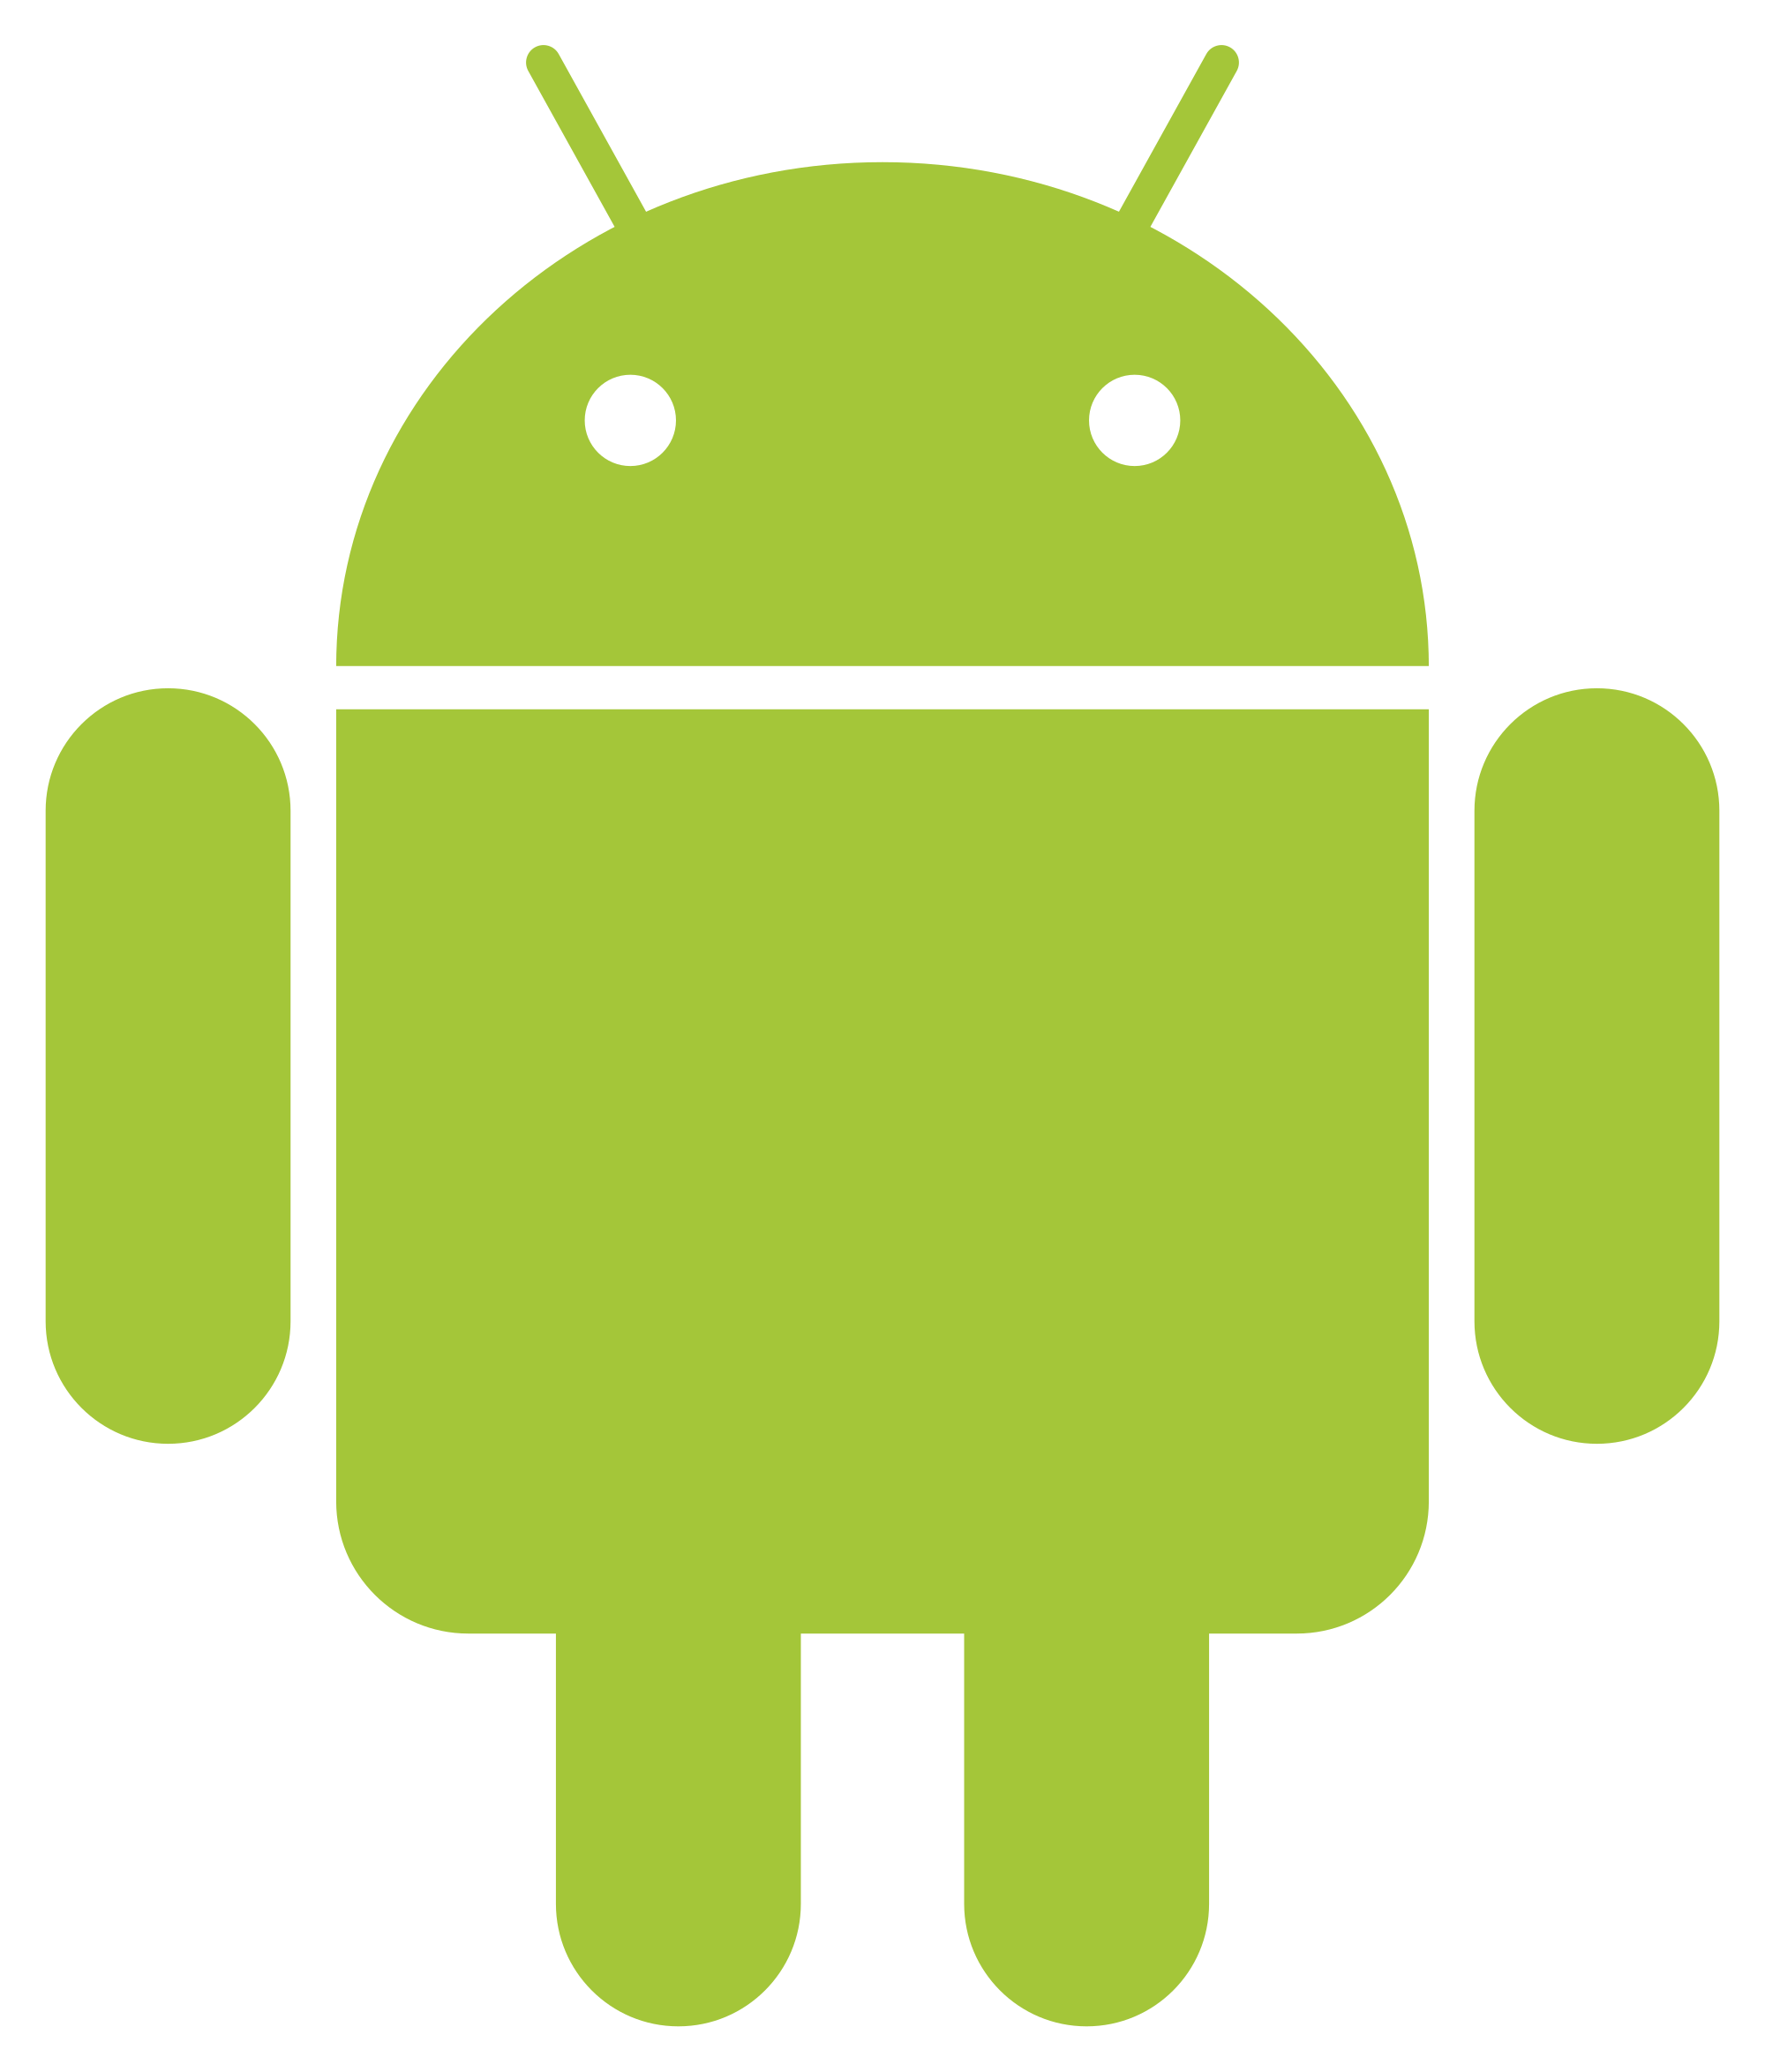
\includegraphics[width=0.1\textwidth]{02/android}
%	\end{center}
%	\caption{Logo Androida}
%\end{figure}

\subsubsection*{Architektura systemu}
Ze względu na architekturę systemu, można wyróżnić w Androidzie kilka abstrakcyjnych warstw: aplikacji, frameworku aplikacji, bibliotek, środowiska wykonawczego i jądra Linux, na którym bazuje cały system. Cała funkcjonalność systemu, niezbędna podczas działania aplikacji, dostępna jest poprzez framework aplikacji, czyli systemowe API napisane w Javie. Używając go, programista może kontrolować sposób działania oraz wygląd programu. Tutaj znajduje się menedżer aktywności (ang. Activity Manager), odpowiedzialny za cykl życia aplikacji, czy menedżer powiadomień (ang. Notification Manager) obsługujący wyświetlanie wszelkich notyfikacji. Także udostępnianie przez aplikacje interfejsów, z wykorzystaniem intencji, możliwe jest dzięki tej warstwie. Poniżej jej znajdują się natywne biblioteki, napisane w C i C++. Dzięki systemowemu API najczęściej nie ma konieczności z nich korzystać, i do tworzenia aplikacji można używać Javy. Najgłębiej w systemie znajduje się jego jądro, czyli Linux. Wykonuje ono najbardziej podstawowe funkcje, będąc odpowiedzialnym m.in. za zarządzanie baterią. Posiada też sterowniki systemowe: ekranu, aparatu, czy audio.
\begin{figure}[h]
	\begin{center}
		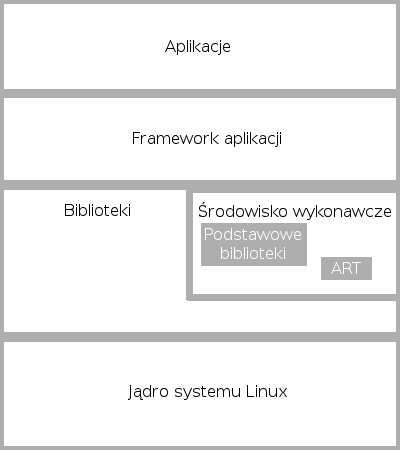
\includegraphics[width=0.5\linewidth]{02/warstwy_android}
	\end{center}
	\caption{Schemat architektury systemu Android}
\end{figure}
\subsubsection*{Środowisko wykonawcze}
Uruchamianiem programów napisanych w Javie zajmuje się wirtualna maszyna Javy (ang. Java Virtual Machine). Po skompilowaniu tworzony jest kod bajtowy, plik \textit{class}, który następnie po załadowaniu interpretowany jest przez JVM (możliwa też kompilacja JIT). Takie podejście pozwala na przenośność programów, czyli niezależność od platformy, kosztem pewnego spadku wydajności.

Mimo, że programy na Androida pisane są w Javie, to nie JVM używany jest do ich późniejszego wykonywana. Głównie jest to spowodowane chęcią stworzenia środowiska uruchomieniowego, które będzie lepiej przystosowane do słabszych wydajnościowo od komputerów maszyn, jakimi są urządzenia mobilne. Proces budowania aplikacji rozpoczyna się tak samo. Kompilator przekształca pliki zawierające kod Javy, do kodu bajtowego. W takiej postaci program nie mógłby zostać jeszcze uruchomiony. Najpierw specjalne narzędzie, pod nazwą \textit{dx}, modyfikuje wynik działania kompilatora. Dla każdej klasy Javy tworzony jest osobny plik \textit{class} - w trakcie działania programu są one ładowne przez JVM. Zadaniem \textit{dx} jest połączenie wszystkich tych kodów bajtowych w jeden plik \textit{dex}, z usunięciem powtarzających się symboli oraz zmianą znajdujących się tam instrukcji, na odpowiednie dla Androida. Dzięki temu skompilowany program będzie mniejszy oraz powinien działać szybciej. Ostatnim etapem budowania aplikacji jest stworzenie pliku \textit{apk}, odpowiednika \textit{jar}, w którym oprócz kodu bajtowego, znajdą się takie zasoby jak zdjęcia wykorzystywane w aplikacji.
\begin{figure}[h]
	\begin{center}
		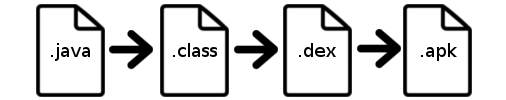
\includegraphics[width=0.5\textwidth]{02/android_dex}
	\end{center}
	\caption{Proces budowy aplikacji}
	\vspace{-0.5cm}
\end{figure}

Do wersji 4.4 Androida (KitKat) aplikacje uruchamiane były w wirtualnej maszynie Dalvik. Sposób działania jest dość zbliżony do JVM. Kod bajtowy w postaci plików \textit{dex} jest interpretowany, z możliwością kompilacji do kodu natywnego (JIT). Jedną z różnic jest sposób działania wirtualnego procesora, który w Dalviku opartu został na rejestrach, a nie na stosie. Takie podejście wpływa na mniejsze zużycie pamięci, jednak programy są większe, gdyż instrukcje muszą zawierać dodatkowe informacje co do rejestrów, z których korzystają.

W wersji 5.0 Androida (Lolipop) zastąpiono dotychczasową maszynę wirtualną Dalvik, środowiskiem uruchomieniowym Android runtime (ART). Również przyjmuje pliki \textit{dex}, jednak nie interpretuje ich, a w momencie instalacji aplikacji - kompiluje. Taka kompilacja kodu pośredniego, języka wysokiego poziomu, do kodu natywnego, nosi nazwę Ahead-of-time (AOT). Przy każdym uruchomieniu aplikacji, dzięki ART, wykorzystywany jest jej natywny kod. Ta zmiana powoduje szybsze działanie i uruchamianie się aplikacji. Wadą jest znacznie dłuższy czas instalacji, który teraz obejmuje także dodatkową kompilację.


\subsubsection*{Programowanie aplikacji}
Aby móc tworzyć aplikacje na Androida z wykorzystaniem Javy, konieczne jest posiadanie:
\begin{itemize}
	\item Java z JDK i JRE,
	\item Android SDK.
\end{itemize}
W ten sposób aplikacja do funkcji systemowych odwoływać się będzie za pomocą udostępnionego przez system API, przeznaczonego dla Javy. Dzięki temu, że nie jest to kod natywny, nie jest konieczna osobna kompilacja dla każdej dostępnej architektury. Programy są uniwersalne i dopiero po zainstalowaniu na konkretnym urządzeniu, interpretowany jest kod bajtowy, bądź przeprowadzana kompilacja AOT. Przez twórców systemu udostępniane jest NDK, czyli Native Development Kit. Z jego pomocą aplikacje mogą być tworzone w C lub C++, odwołując się bezpośrednio do bibliotek systemowych. Niestety, mimo możliwego zysku na wydajności, stworzony kod jest zależny od architektury. Dodatkowo większość zewnętrznych bibliotek jest tworzonych w Javie. 

Bardzo zalecane jest używanie zintegrowanego środowiska programistycznego, które automatyzuje niektóre czynności. Potrafi stworzyć za użytkownika projekt z wymaganą strukturą plików, wykonać wszystkie etapy kompilacji, wgrać program na urządzenie i wiele innych. Dedykowanym IDE jest Android Studio, do niedawna wykorzystywany był domyślnie Eclipse.

\begin{figure}[h]
	\begin{center}
		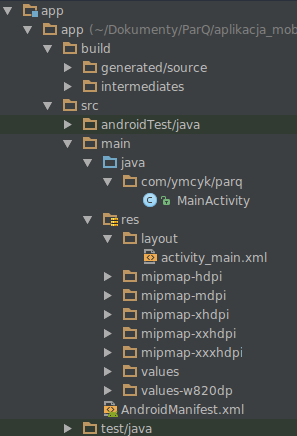
\includegraphics[width=0.25\textwidth]{02/android_pliki}
	\end{center}
	\caption{Pliki projektu utworzonego w Android Studio}
	\vspace{-0.3cm}
\end{figure}
Podczas działania aplikacja prezentuje użytkownikowi tzw. ekrany. Są to odpowiedniki okien systemowych, gdzie umieszczane są elementy graficznego interfejsu użytkownika, czyli widoki (ang. views), jak np.: przyciski, rozwijane listy, czy pola tekstowe. Wchodząc z nimi w interakcję (poprzez dotyk, w ekranach dotykowych), możliwa jest komunikacja między użytkownikiem, a urządzeniem. 

Wygląd ekranów definiowany jest w plikach XML, nazywanych układami (ang. layout). Każdy z widoków jest osobnym znacznikiem, a za pomocą argumentów można modyfikować wybrane parametry jak rozmiar, czy kolor. Wszystkie widoki w pliku XML muszą posiadać swojego rodzica, który definiuje jak mają one być traktowane w tym układzie. W Androidzie można skorzystać z trzech. RelativeLayout - położenie widoków określane jest względem siebie. LinearLayout - układ liniowy, gdzie elementy GUI wyświetlane są jeden koło drugiego. GridLayout - dzieli ekran na siatkę, składającą się z wierszy oraz kolumn, i pozwala umieścić widoki we wskazanych komórkach.

Układy definiują jak dany ekran ma wyglądać, natomiast aktywności (ang. activity), czyli klasy Javy, określają w jaki sposób mają one reagować na interakcje użytkownika. Przechodząc do danego ekranu, tworzona jest najpierw aktywność. W metodzie onCreate, wywoływanej przed wyświetleniem ekranu, wybierany jest układ, który ma zostać użyty przez system do stworzenia interfejsu. Widoki z tego układu mogą mieć powiązane ze sobą jakieś operacje, które będą przeprowadzane np.: po naciśnięciu przycisku. To także odbywa się w aktywności, która może posiadać metody wywoływane po zakończeniu danej interakcji.

\subsubsection*{Podsumowanie}
Rozwiązania mobilne cieszą się coraz większym zainteresowaniem. Tylko w sklepie z aplikacjami Androida, Google Play, liczba programów przekroczyła w 2015 r. 1,6 mln \cite{biblia_ebiznesu_2}. Powstające coraz to nowe urządzenia, na których zainstalowany jest Android sprawia, że umiejętność programowania na tą platformę będzie coraz bardziej doceniana.


\subsection{Aplikacja internetowa w Django}
% wprowadzenie o tym, że frameworki nadają się do różnych zadań